\ifpdf
    \graphicspath{{Appendix3/Appendix3Figs/PNG/}{Appendix3/Appendix3Figs/PDF/}{Appendix3/Appendix3Figs/}}
\else
    \graphicspath{{Appendix3/Appendix3Figs/EPS/}{Appendix3/Appendix3Figs/}}
\fi  

\section{Eye-gaze visualisations} \label{appdx:eyegaze}

\begin{figure}[!htb]
\centering
\begin{subfigure}{.5\textwidth}
  \centering
  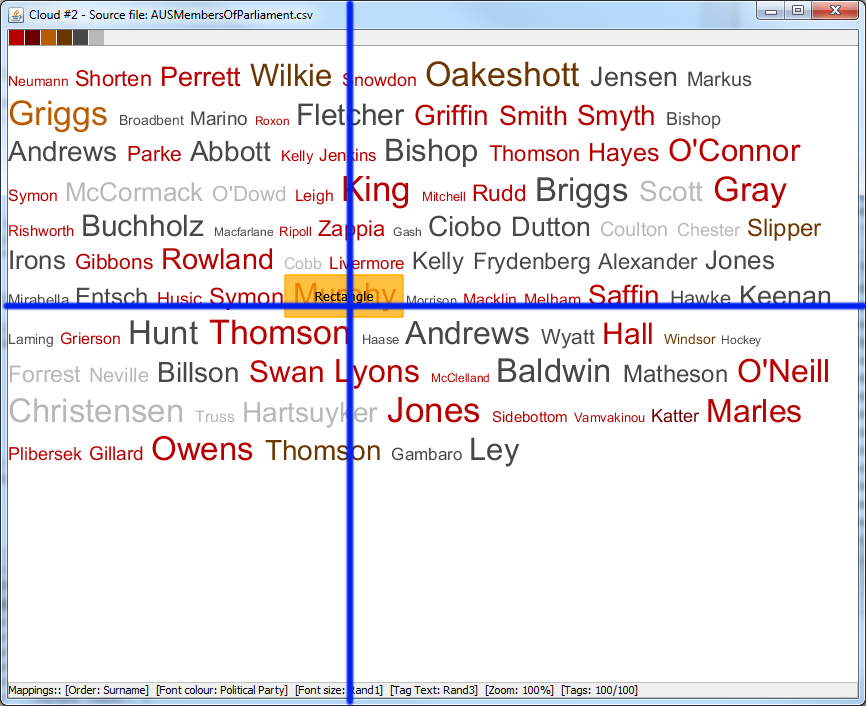
\includegraphics[scale=0.25]{Experiment1/Trial1/C2S2L2.png}
\end{subfigure}%
\begin{subfigure}{.5\textwidth}
  \centering
  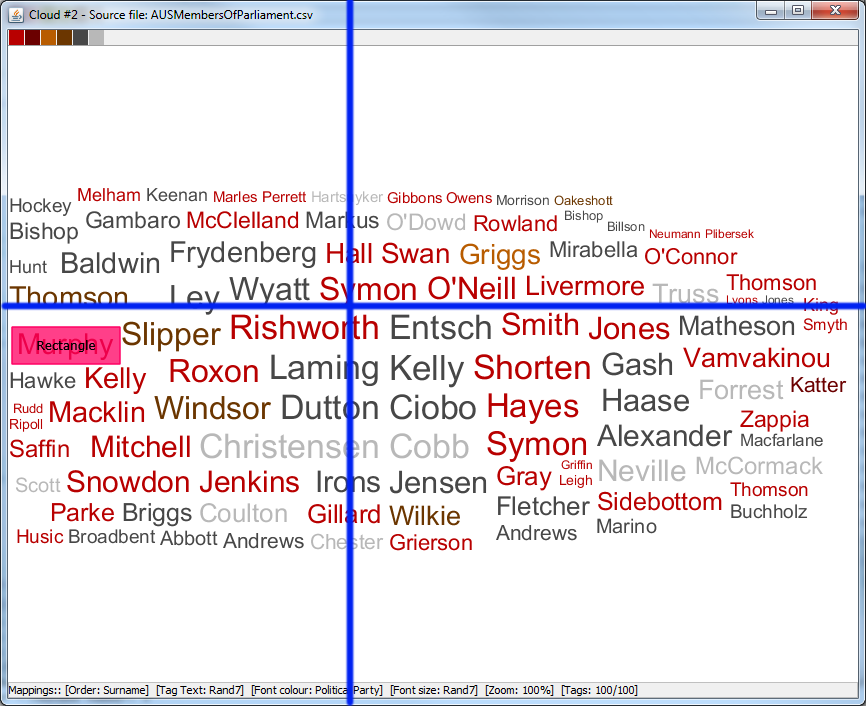
\includegraphics[scale=0.25]{Experiment1/Trial1/C2S2L1.png}
\end{subfigure}
\begin{subfigure}{.5\textwidth}
  \centering
  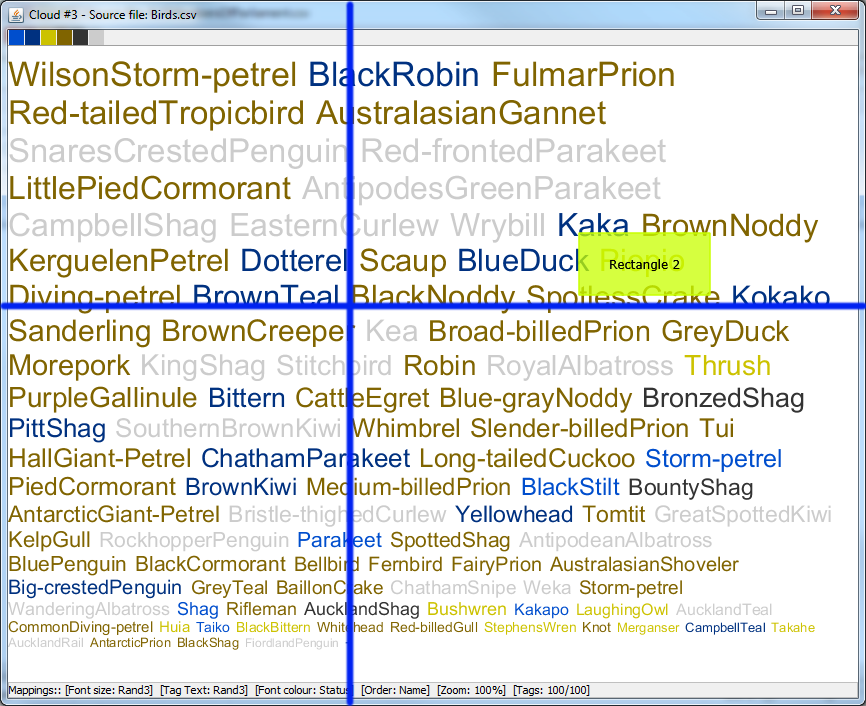
\includegraphics[scale=0.25]{Experiment1/Trial2/C2S2L2.png}
\end{subfigure}%
\begin{subfigure}{.5\textwidth}
  \centering
 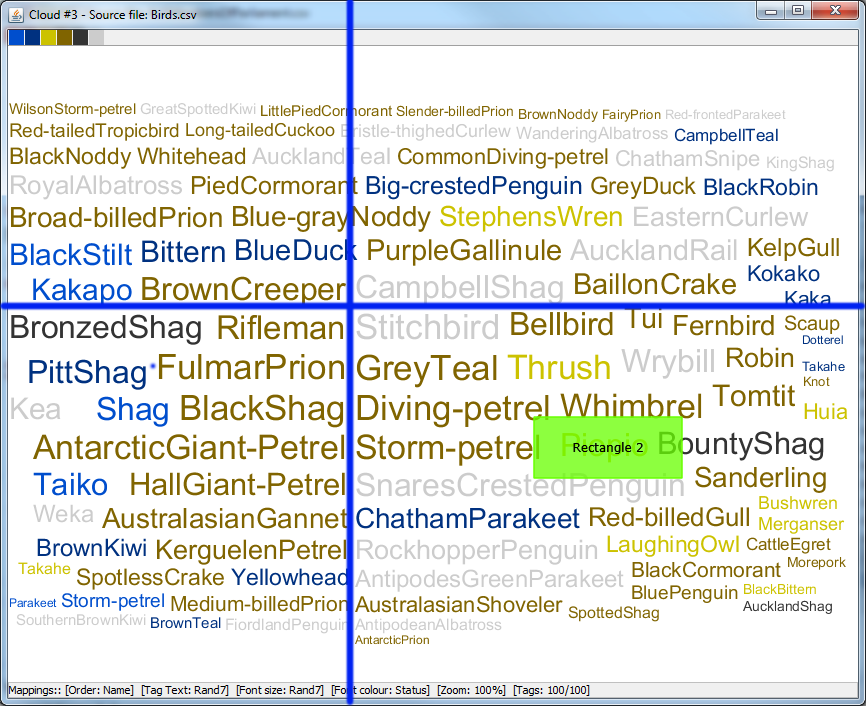
\includegraphics[scale=0.25]{Experiment1/Trial2/C2S2L1.png}
\end{subfigure}
\begin{subfigure}{.5\textwidth}
  \centering
  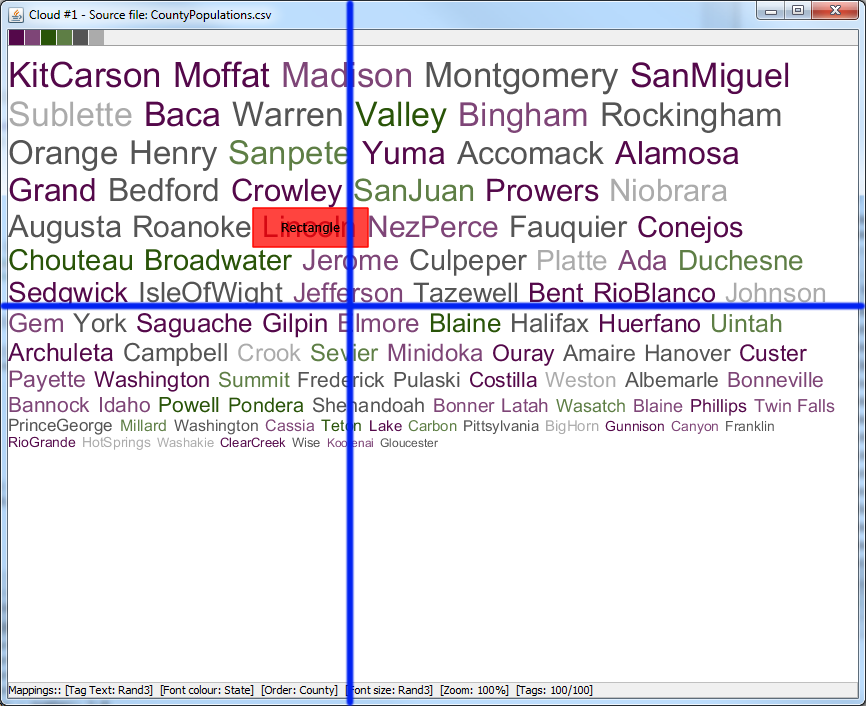
\includegraphics[scale=0.25]{Experiment1/Trial3/C2S2L2.png}
\end{subfigure}%
\begin{subfigure}{.5\textwidth}
  \centering
 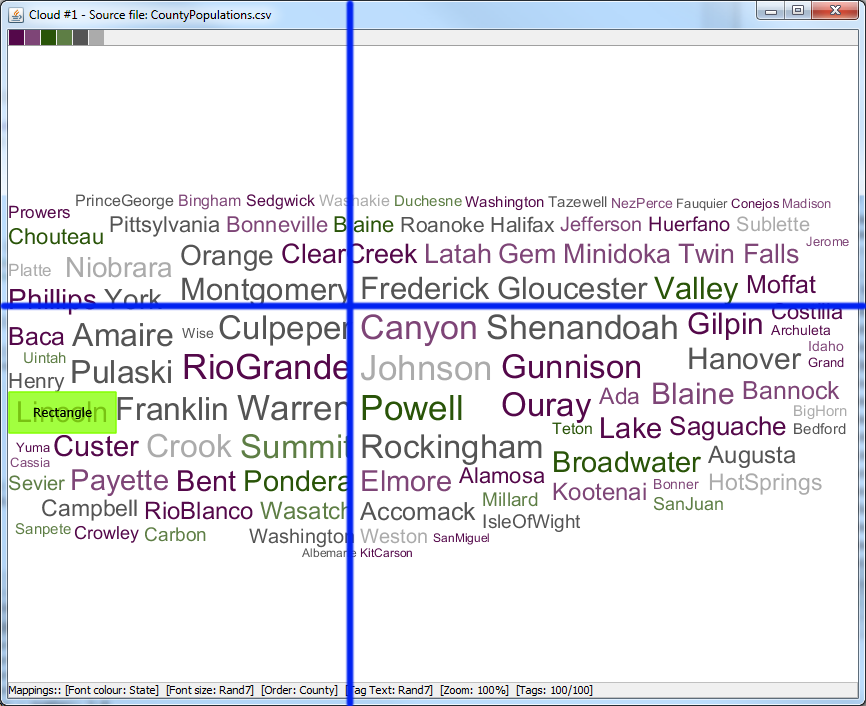
\includegraphics[scale=0.25]{Experiment1/Trial3/C2S2L1.png}
\end{subfigure}
\begin{subfigure}{.5\textwidth}
  \centering
  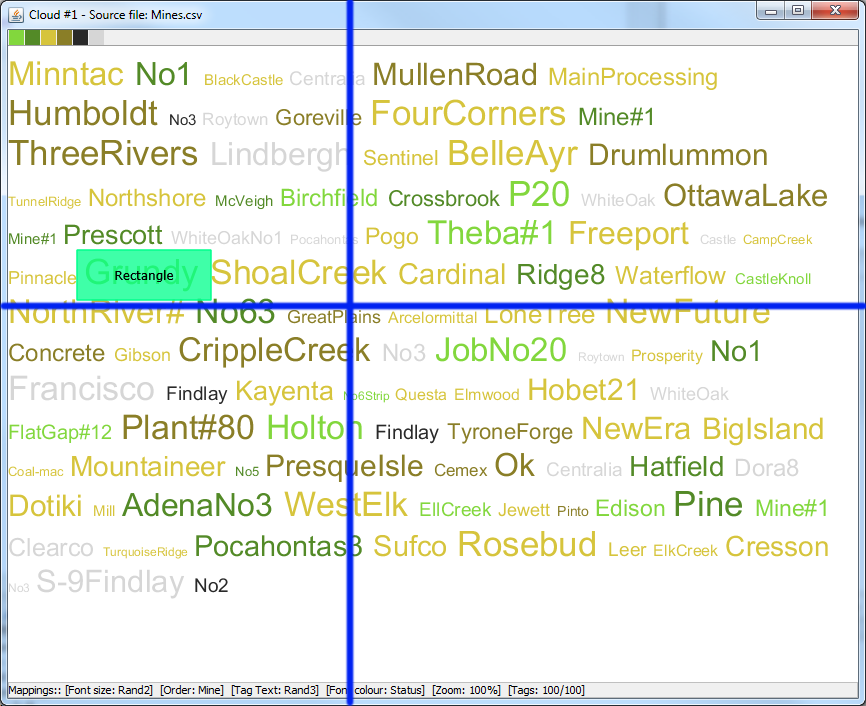
\includegraphics[scale=0.25]{Experiment1/Trial4/C2S2L2.png}
\end{subfigure}%
\begin{subfigure}{.5\textwidth}
  \centering
 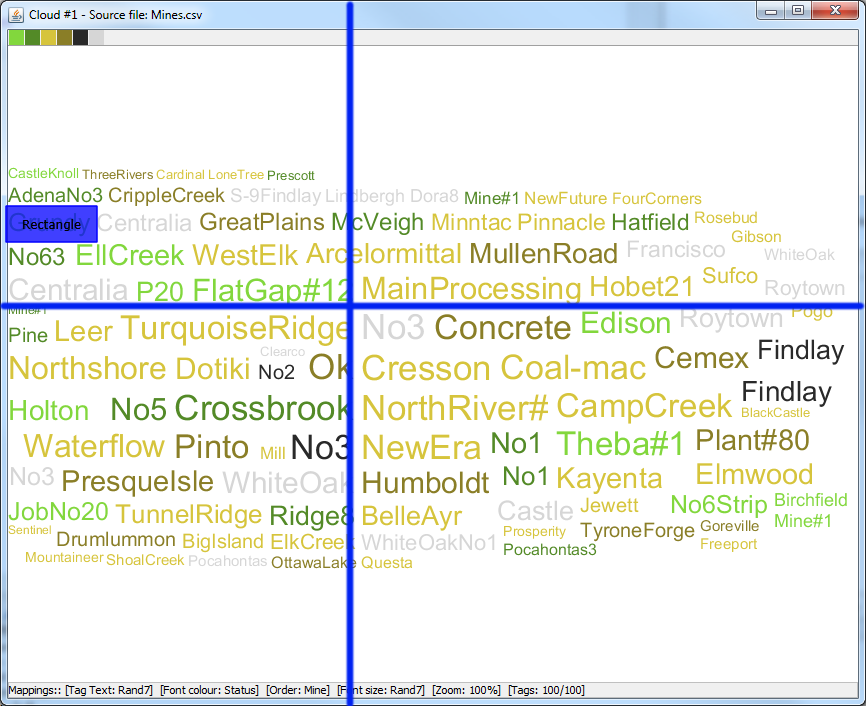
\includegraphics[scale=0.25]{Experiment1/Trial4/C2S2L1.png}
\end{subfigure}
\caption{\textit{Experiment one: foreground colour with large target, typewriter and spiral layout}}
\label{fig:target1}
\end{figure}

\begin{figure}[!htb]
\centering
\begin{subfigure}{.5\textwidth}
  \centering
  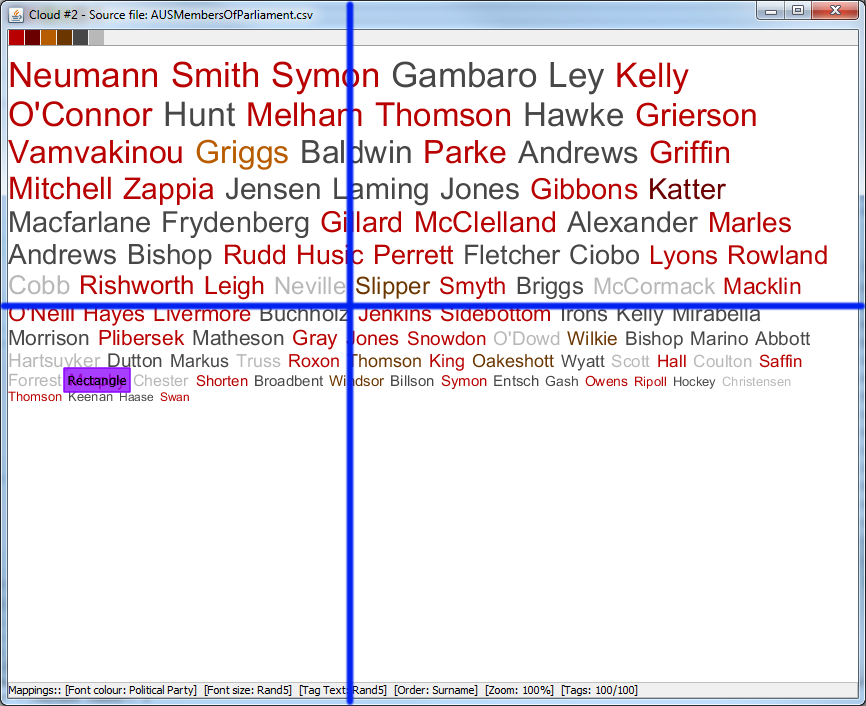
\includegraphics[scale=0.25]{Experiment1/Trial1/C2S1L2.png}
\end{subfigure}%
\begin{subfigure}{.5\textwidth}
  \centering
  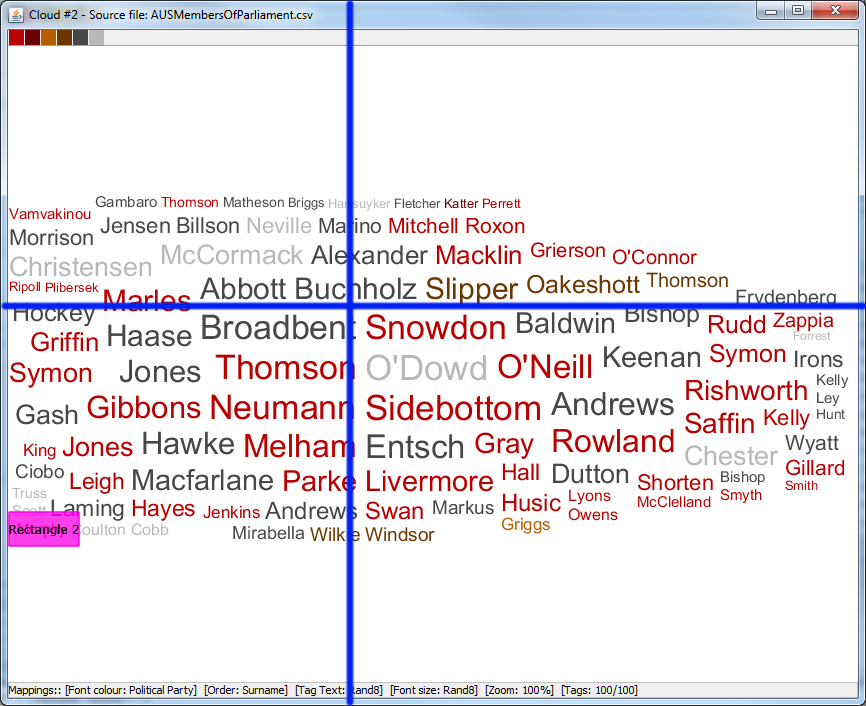
\includegraphics[scale=0.25]{Experiment1/Trial1/C2S1L1.png}
\end{subfigure}
\begin{subfigure}{.5\textwidth}
  \centering
  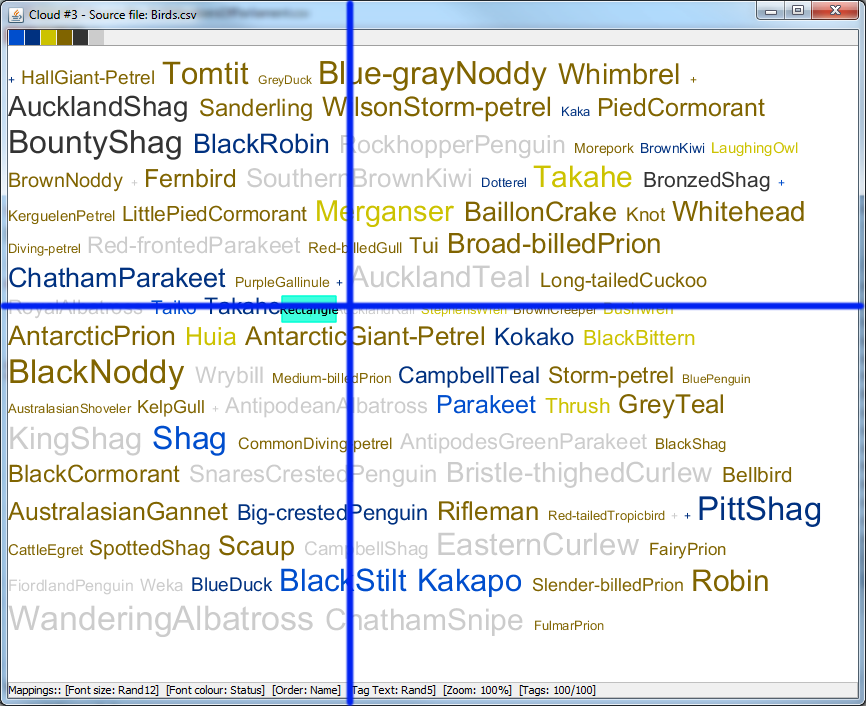
\includegraphics[scale=0.25]{Experiment1/Trial2/C2S1L2.png}
\end{subfigure}%
\begin{subfigure}{.5\textwidth}
  \centering
 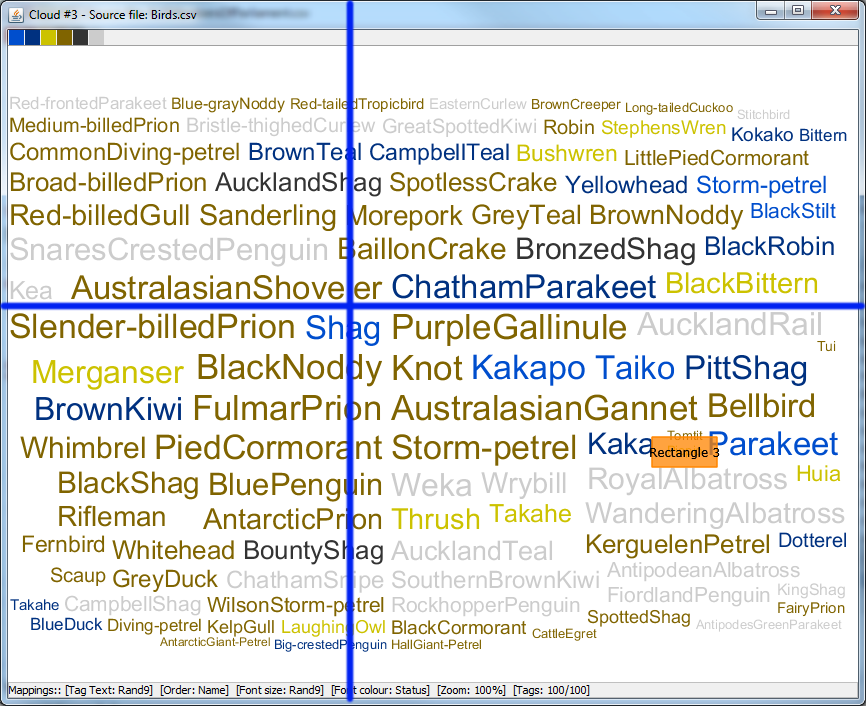
\includegraphics[scale=0.25]{Experiment1/Trial2/C2S1L1.png}
\end{subfigure}
\begin{subfigure}{.5\textwidth}
  \centering
  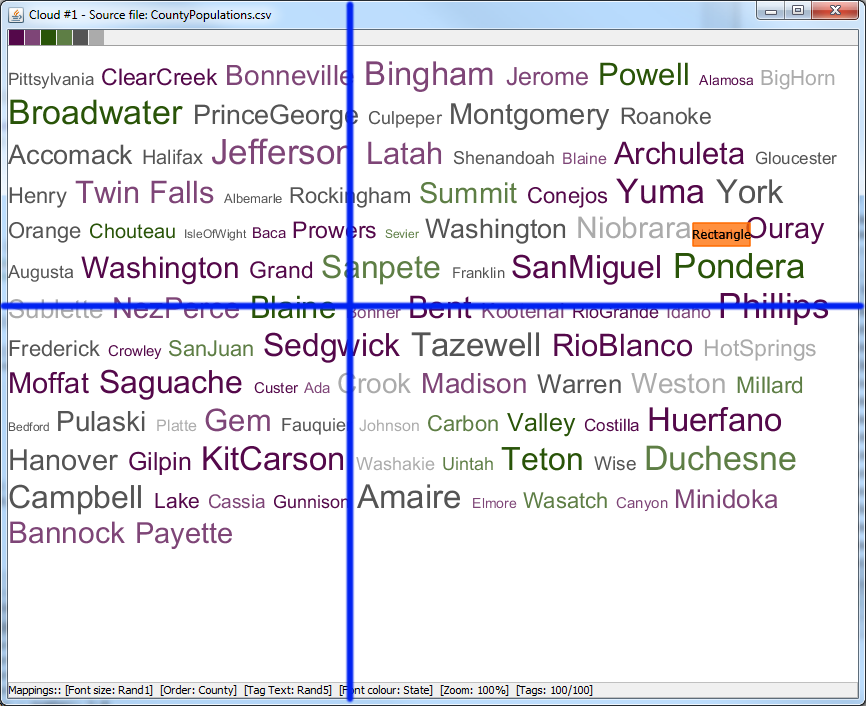
\includegraphics[scale=0.25]{Experiment1/Trial3/C2S1L2.png}
\end{subfigure}%
\begin{subfigure}{.5\textwidth}
  \centering
 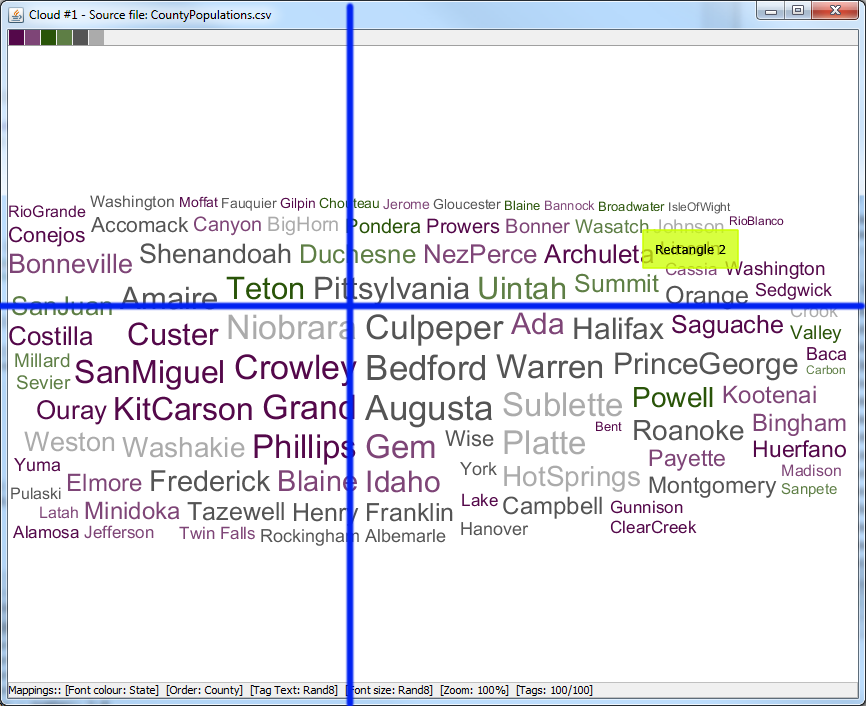
\includegraphics[scale=0.25]{Experiment1/Trial3/C2S1L1.png}
\end{subfigure}
\begin{subfigure}{.5\textwidth}
  \centering
  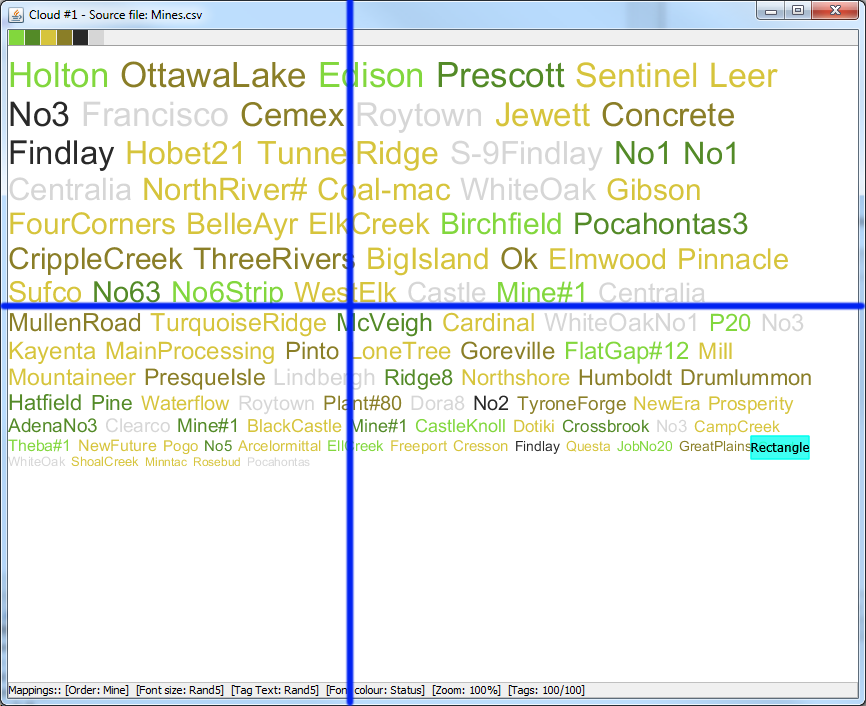
\includegraphics[scale=0.25]{Experiment1/Trial4/C2S1L2.png}
\end{subfigure}%
\begin{subfigure}{.5\textwidth}
  \centering
 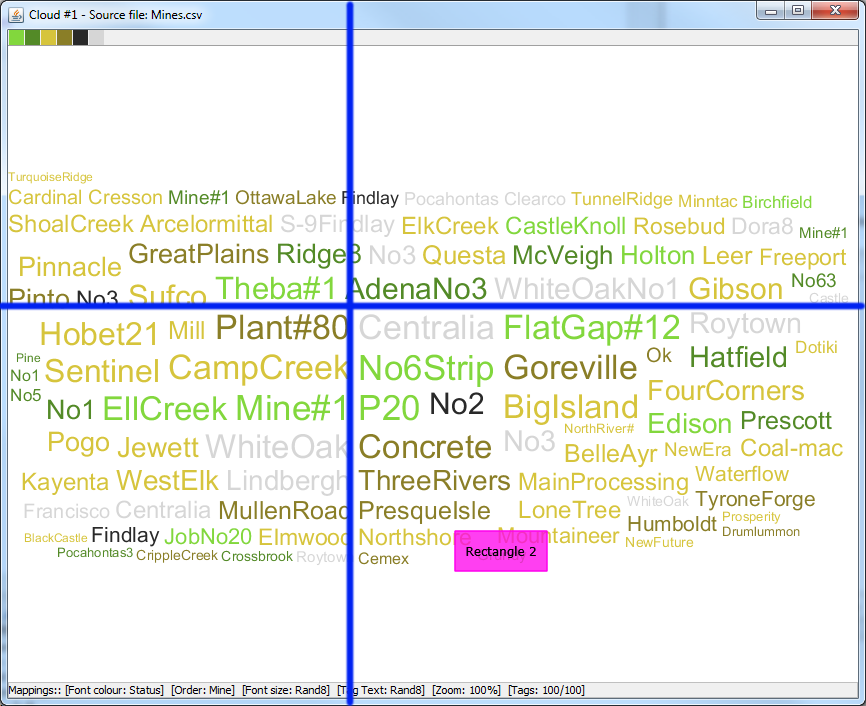
\includegraphics[scale=0.25]{Experiment1/Trial4/C2S1L1.png}
\end{subfigure}
\caption{\textit{Experiment one: foreground colour with small target, typewriter and spiral layout}}
\label{fig:target2}
\end{figure}

\begin{figure}[!htb]
\centering
\begin{subfigure}{.5\textwidth}
  \centering
  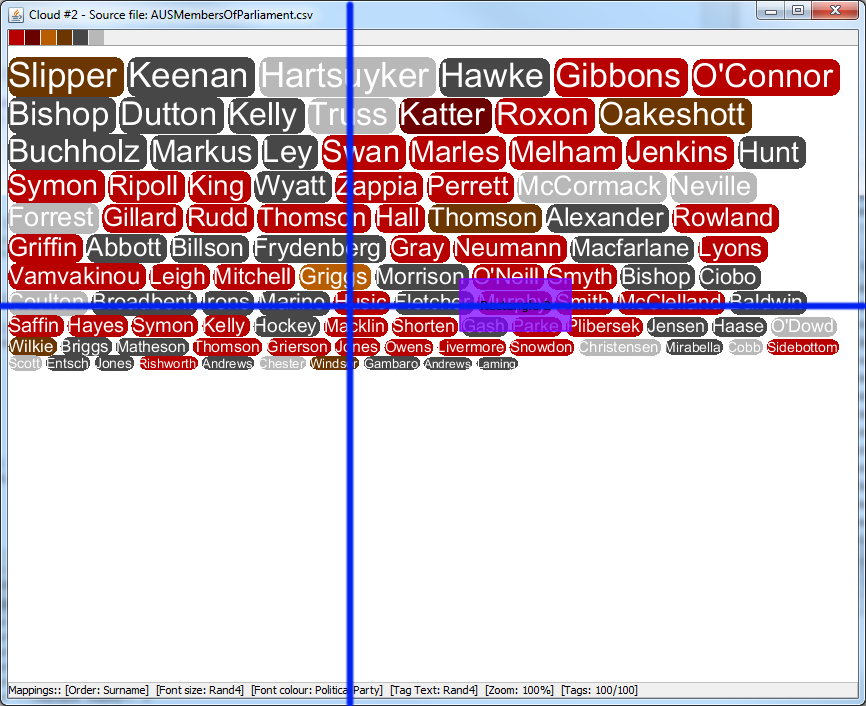
\includegraphics[scale=0.25]{Experiment1/Trial1/C1S1L2.png}
\end{subfigure}%
\begin{subfigure}{.5\textwidth}
  \centering
  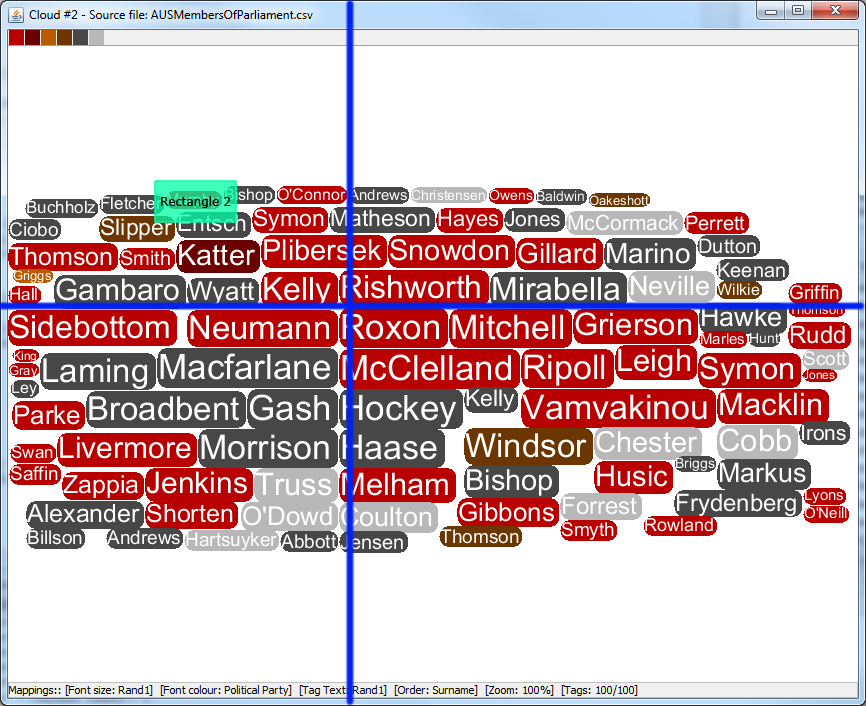
\includegraphics[scale=0.25]{Experiment1/Trial1/C1S1L1.png}
\end{subfigure}
\begin{subfigure}{.5\textwidth}
  \centering
  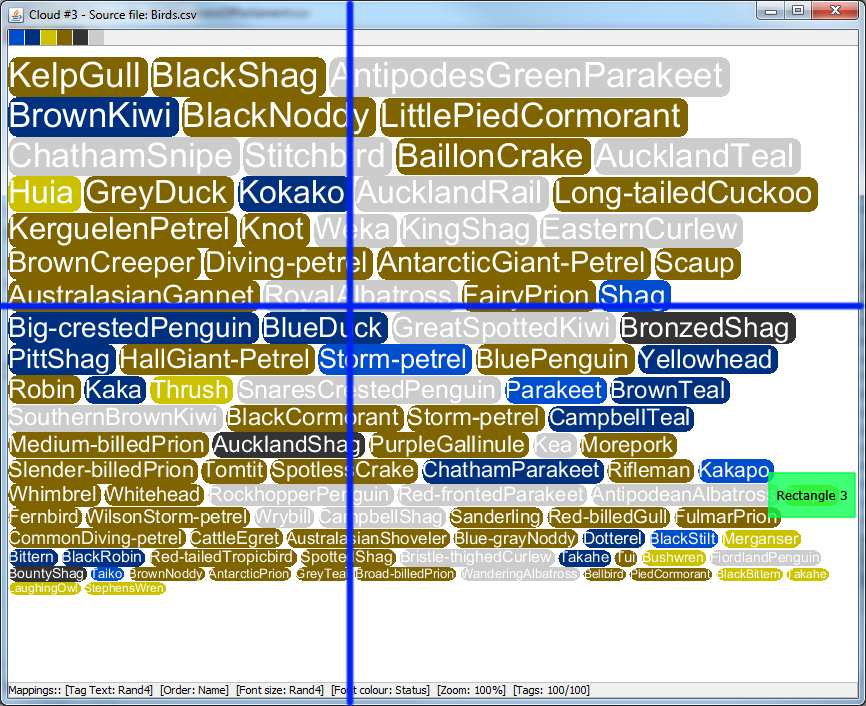
\includegraphics[scale=0.25]{Experiment1/Trial2/C1S1L2.png}
\end{subfigure}%
\begin{subfigure}{.5\textwidth}
  \centering
 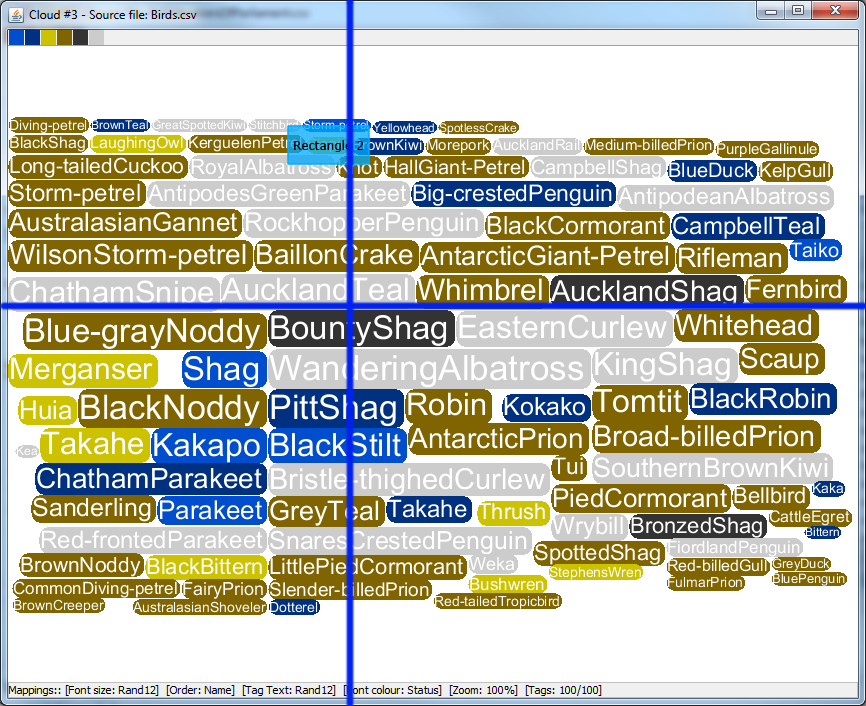
\includegraphics[scale=0.25]{Experiment1/Trial2/C1S1L1.png}
\end{subfigure}
\begin{subfigure}{.5\textwidth}
  \centering
  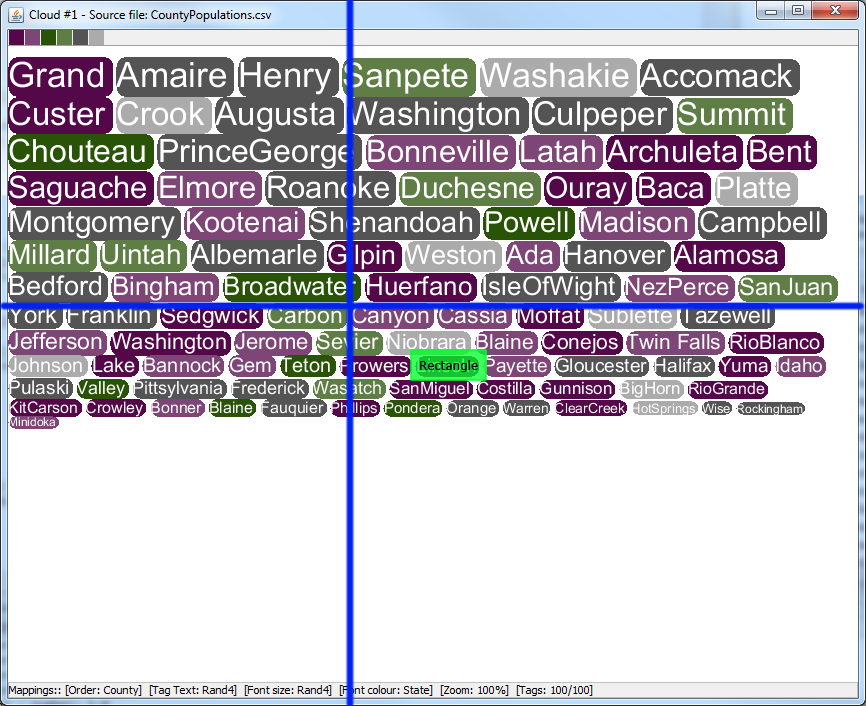
\includegraphics[scale=0.25]{Experiment1/Trial3/C1S1L2.png}
\end{subfigure}%
\begin{subfigure}{.5\textwidth}
  \centering
 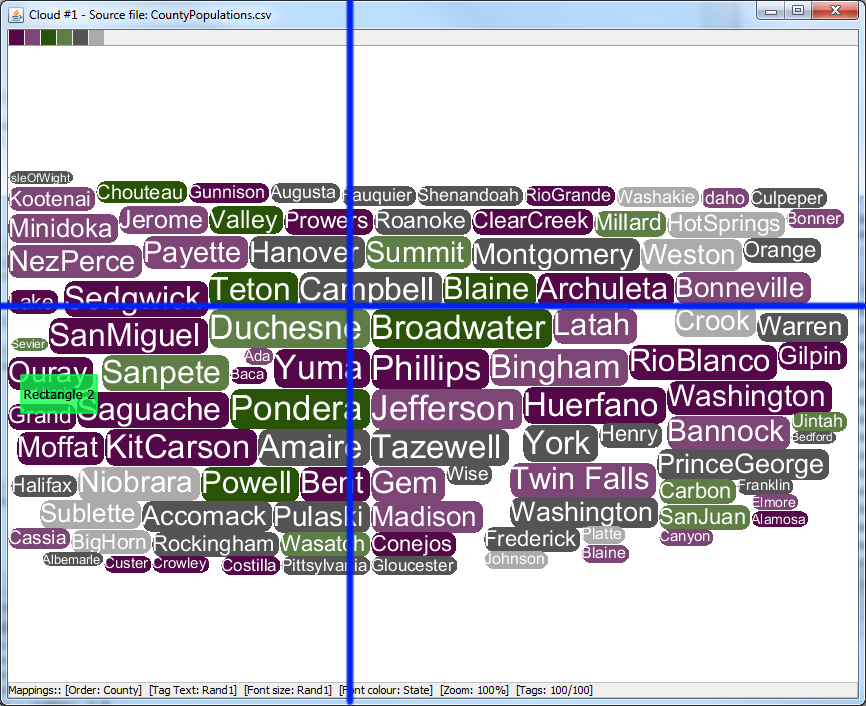
\includegraphics[scale=0.25]{Experiment1/Trial3/C1S1L1.png}
\end{subfigure}
\begin{subfigure}{.5\textwidth}
  \centering
  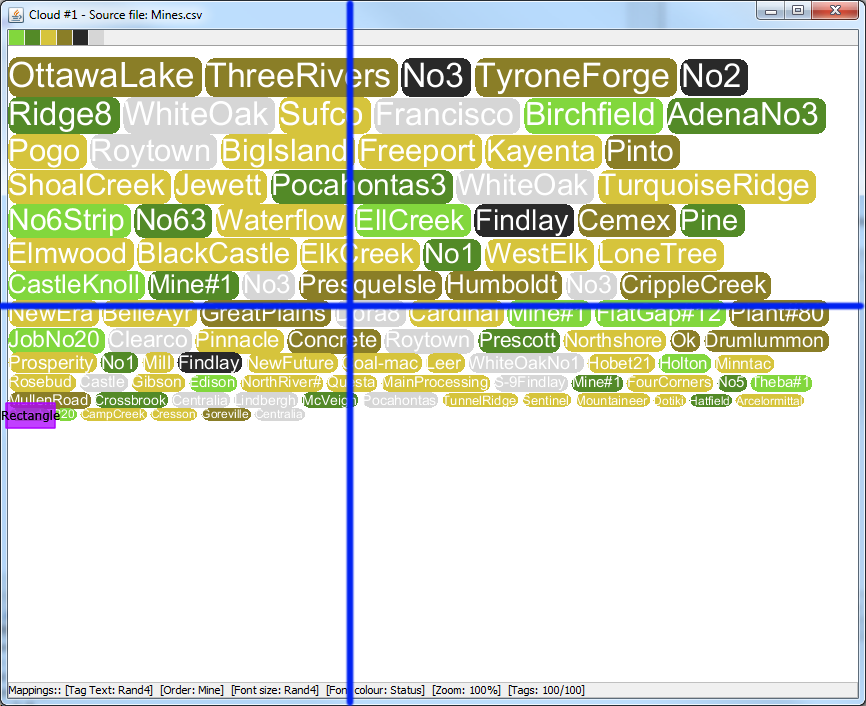
\includegraphics[scale=0.25]{Experiment1/Trial4/C1S1L2.png}
\end{subfigure}%
\begin{subfigure}{.5\textwidth}
  \centering
 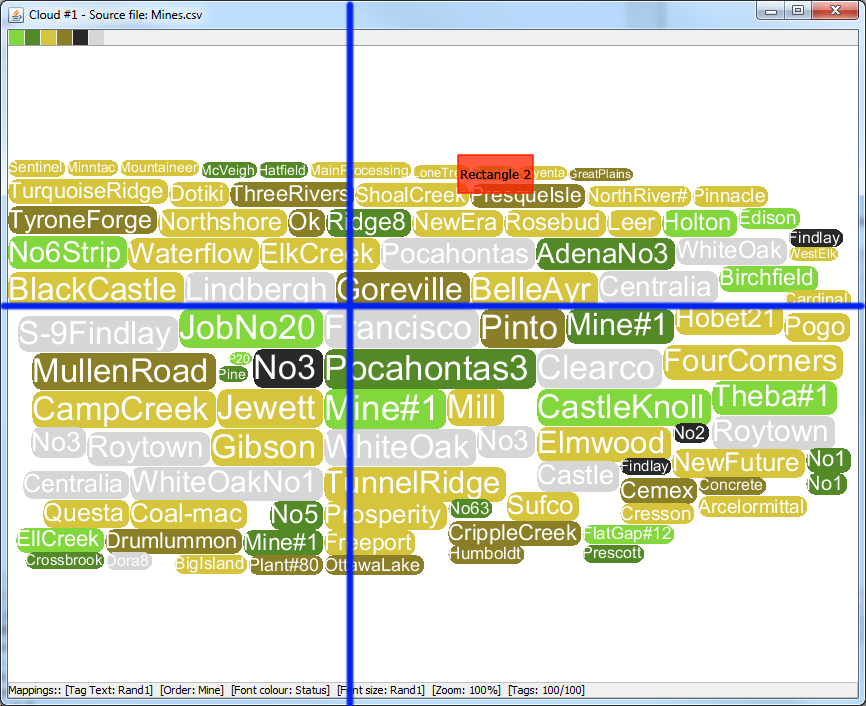
\includegraphics[scale=0.25]{Experiment1/Trial4/C1S1L1.png}
\end{subfigure}
\caption{\textit{Experiment one: background colour with small target, typewriter and spiral layout}}
\label{fig:target3}
\end{figure}



\begin{figure}[!htb]
\centering
\begin{subfigure}{.5\textwidth}
  \centering
  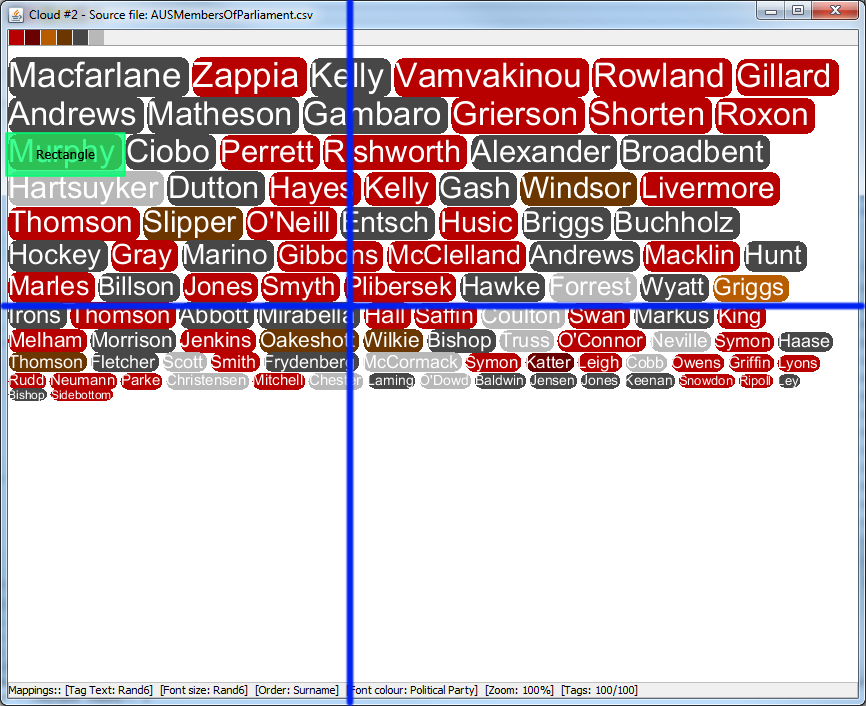
\includegraphics[scale=0.25]{Experiment1/Trial1/C1S2L2.png}
\end{subfigure}%
\begin{subfigure}{.5\textwidth}
  \centering
  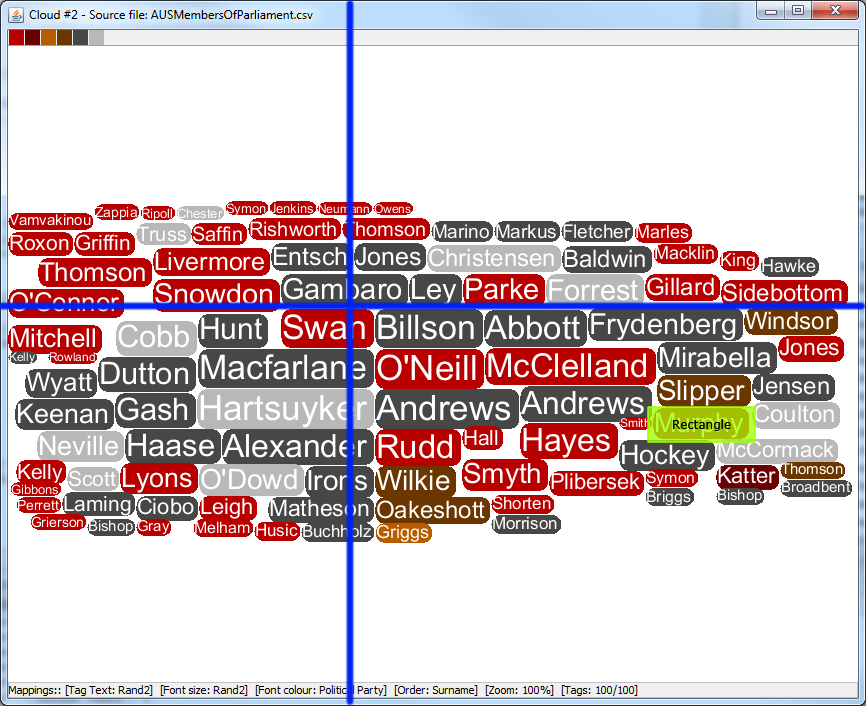
\includegraphics[scale=0.25]{Experiment1/Trial1/C1S2L1.png}
\end{subfigure}
\begin{subfigure}{.5\textwidth}
  \centering
  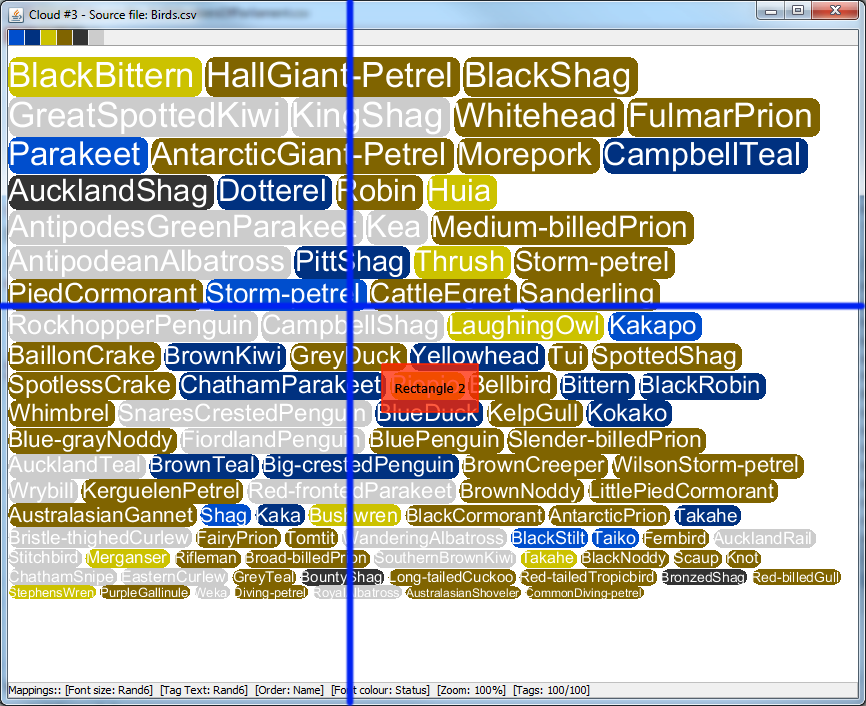
\includegraphics[scale=0.25]{Experiment1/Trial2/C1S2L2.png}
\end{subfigure}%
\begin{subfigure}{.5\textwidth}
  \centering
 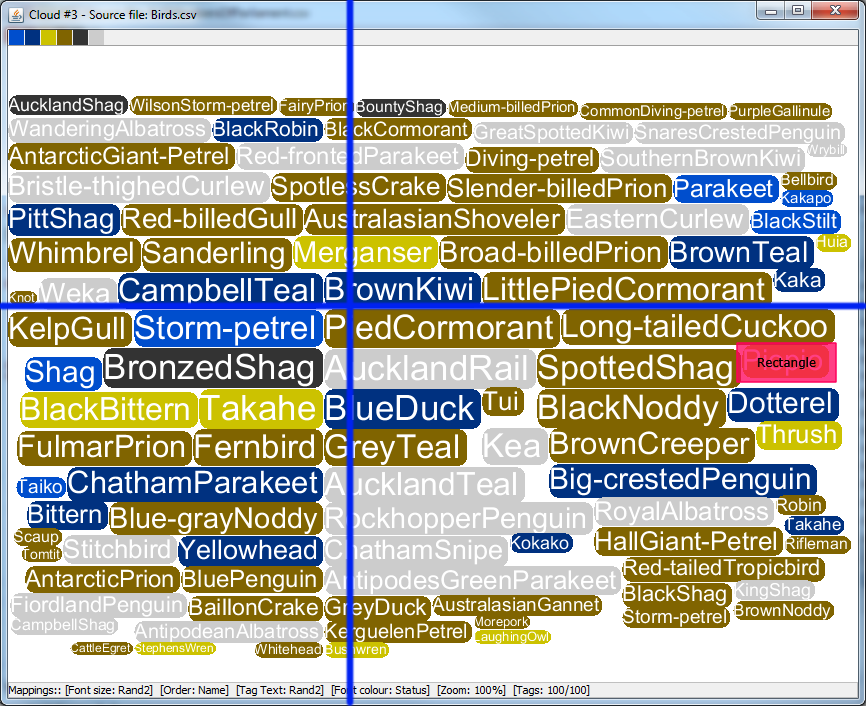
\includegraphics[scale=0.25]{Experiment1/Trial2/C1S2L1.png}
\end{subfigure}
\begin{subfigure}{.5\textwidth}
  \centering
  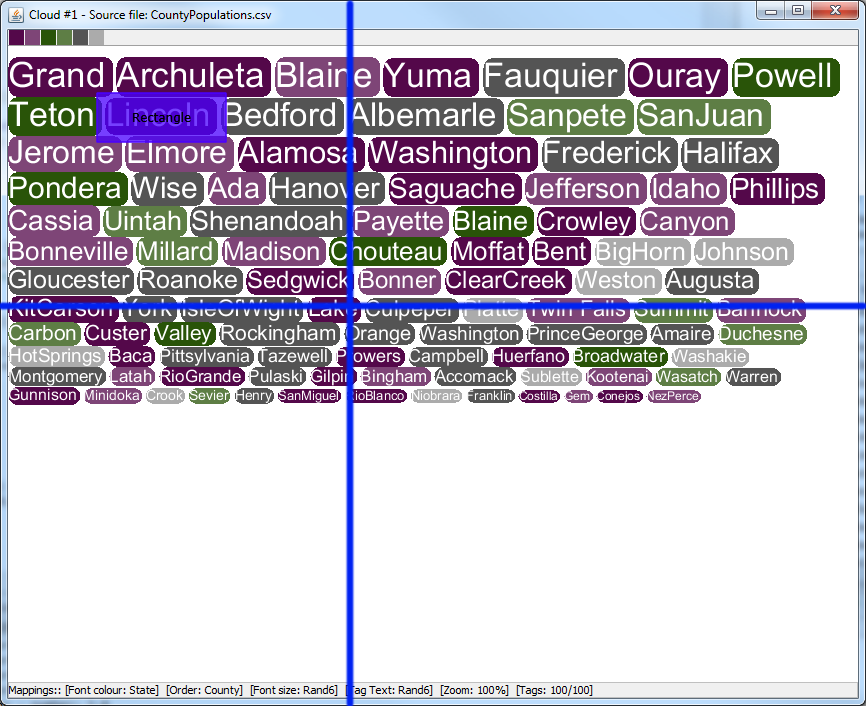
\includegraphics[scale=0.25]{Experiment1/Trial3/C1S2L2.png}
\end{subfigure}%
\begin{subfigure}{.5\textwidth}
  \centering
 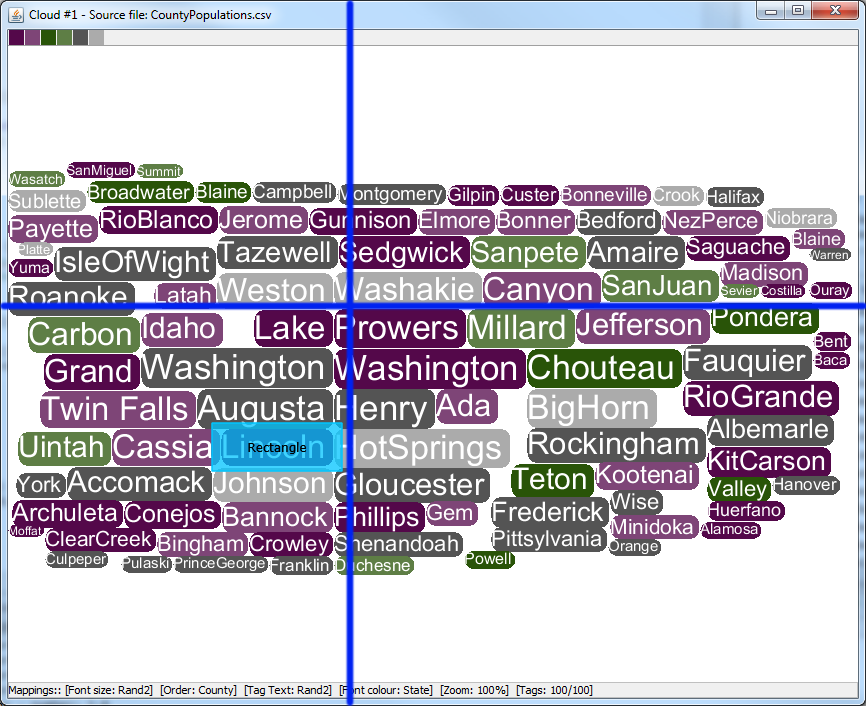
\includegraphics[scale=0.25]{Experiment1/Trial3/C1S2L1.png}
\end{subfigure}
\begin{subfigure}{.5\textwidth}
  \centering
  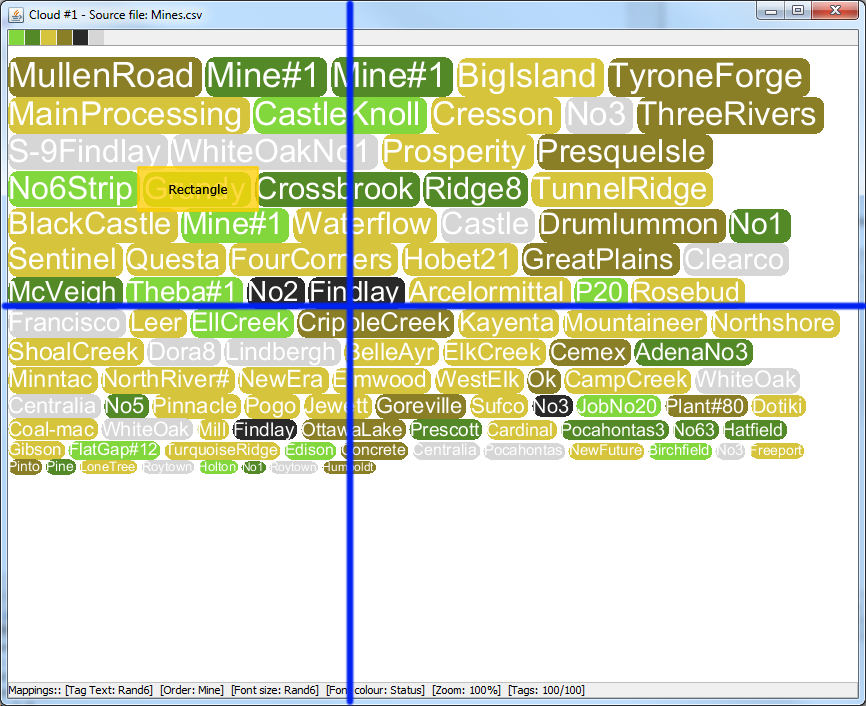
\includegraphics[scale=0.25]{Experiment1/Trial4/C1S2L2.png}
\end{subfigure}%
\begin{subfigure}{.5\textwidth}
  \centering
 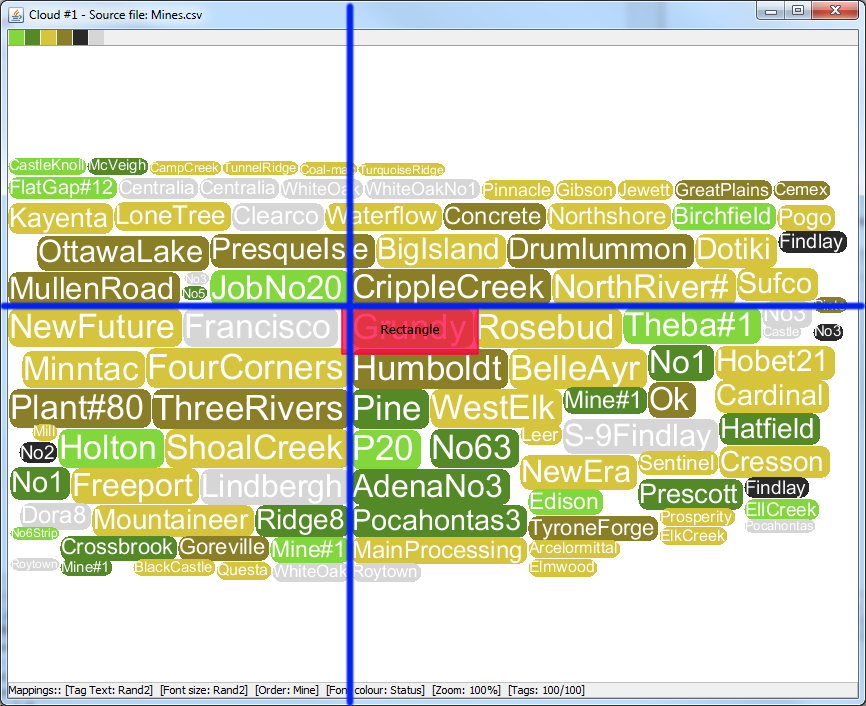
\includegraphics[scale=0.25]{Experiment1/Trial4/C1S2L1.png}
\end{subfigure}
\caption{\textit{Experiment one: background colour with small target, typewriter and spiral layout}}
\label{fig:target4}
\end{figure}

\begin{figure}[!htb]
\centering
\begin{subfigure}{.5\textwidth}
  \centering
  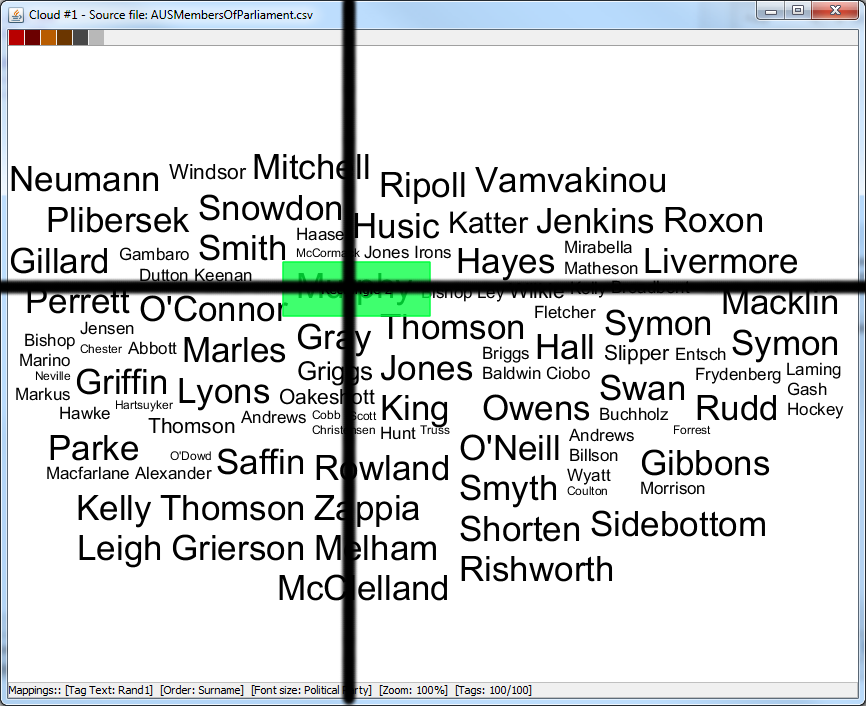
\includegraphics[scale=0.25]{Experiment2/T1/M1Spiral.png}
\end{subfigure}%
\begin{subfigure}{.5\textwidth}
  \centering
  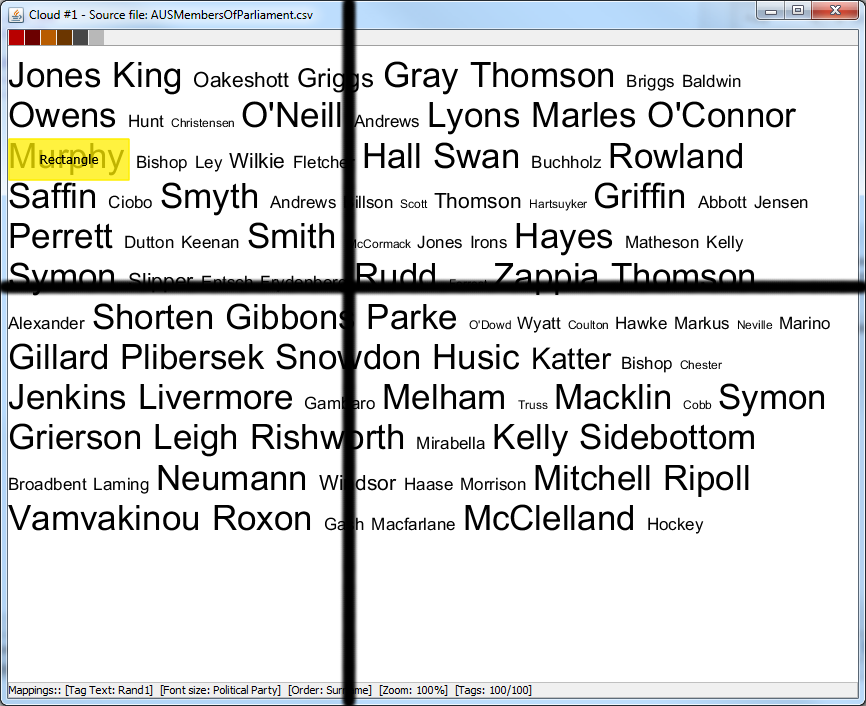
\includegraphics[scale=0.25]{Experiment2/T1/M1Typewriter.png}
\end{subfigure}
\begin{subfigure}{.5\textwidth}
  \centering
  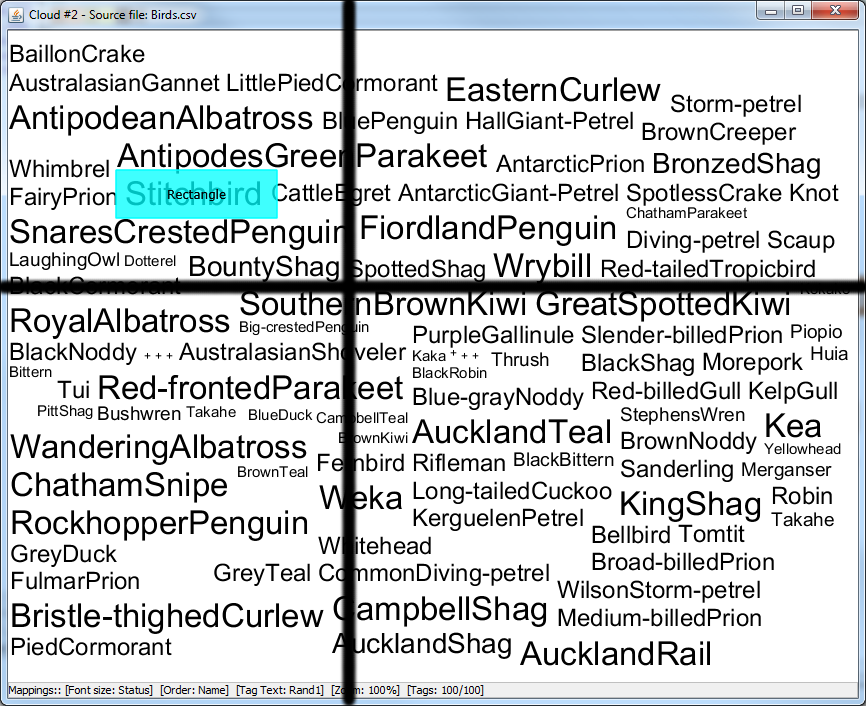
\includegraphics[scale=0.25]{Experiment2/T2/M1Spiral.png}
\end{subfigure}%
\begin{subfigure}{.5\textwidth}
  \centering
  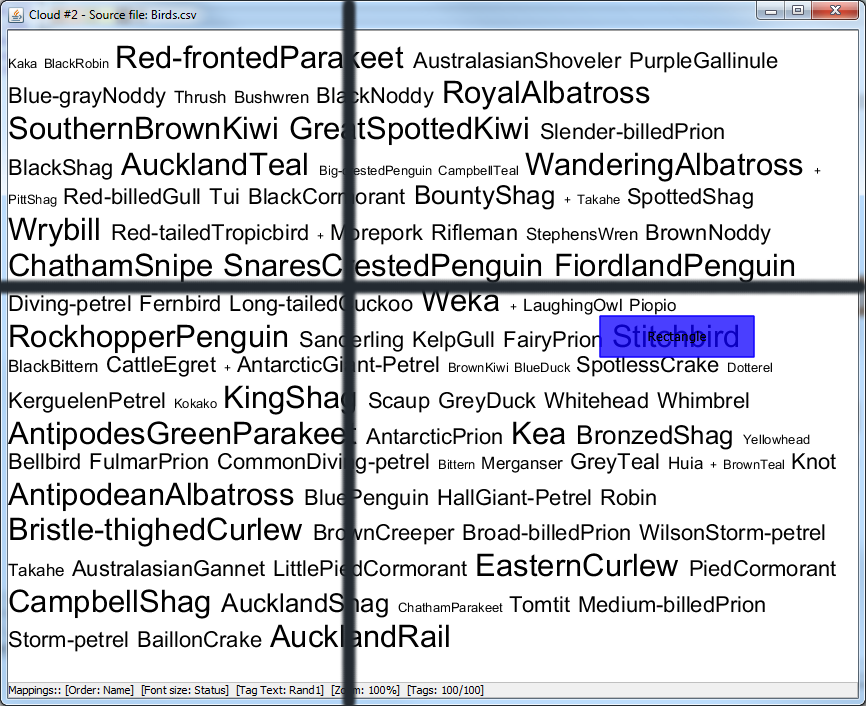
\includegraphics[scale=0.25]{Experiment2/T2/M1Typewriter.png}
\end{subfigure}
\begin{subfigure}{.5\textwidth}
  \centering
  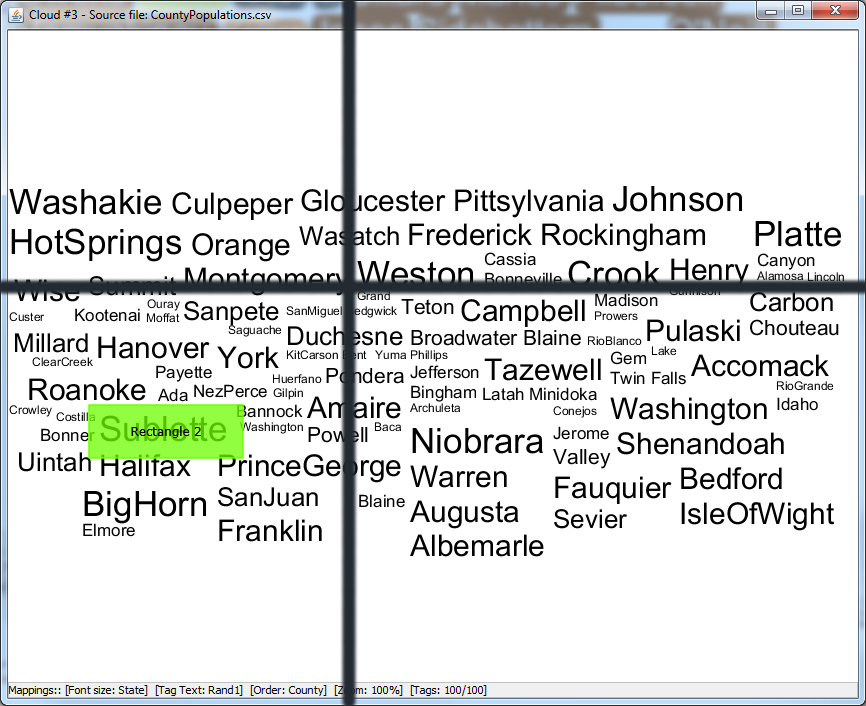
\includegraphics[scale=0.25]{Experiment2/T3/M1Spiral.png}
\end{subfigure}%
\begin{subfigure}{.5\textwidth}
  \centering
  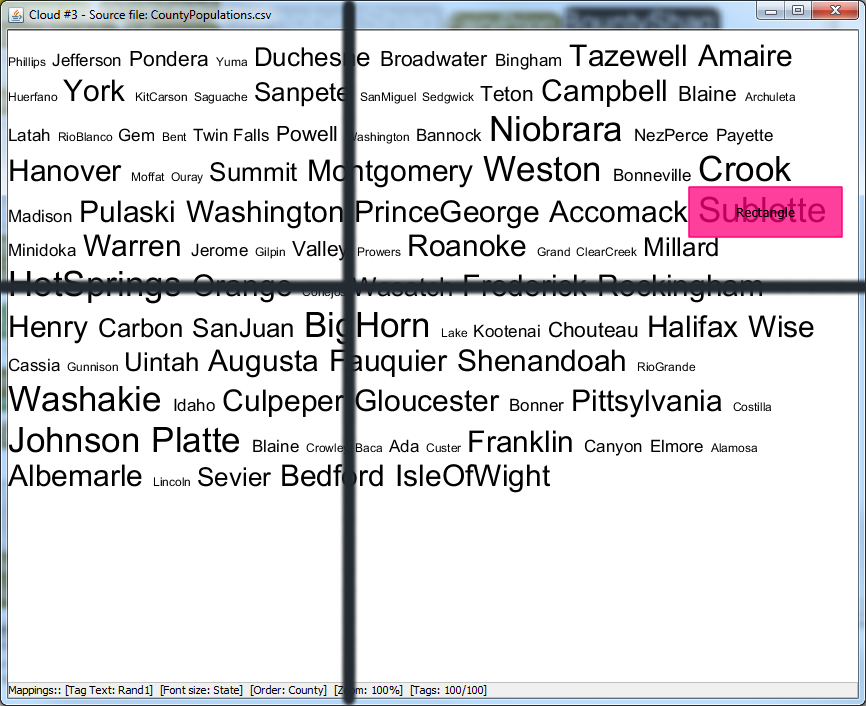
\includegraphics[scale=0.25]{Experiment2/T3/M1Typewriter.png}
\end{subfigure}
\begin{subfigure}{.5\textwidth}
  \centering
  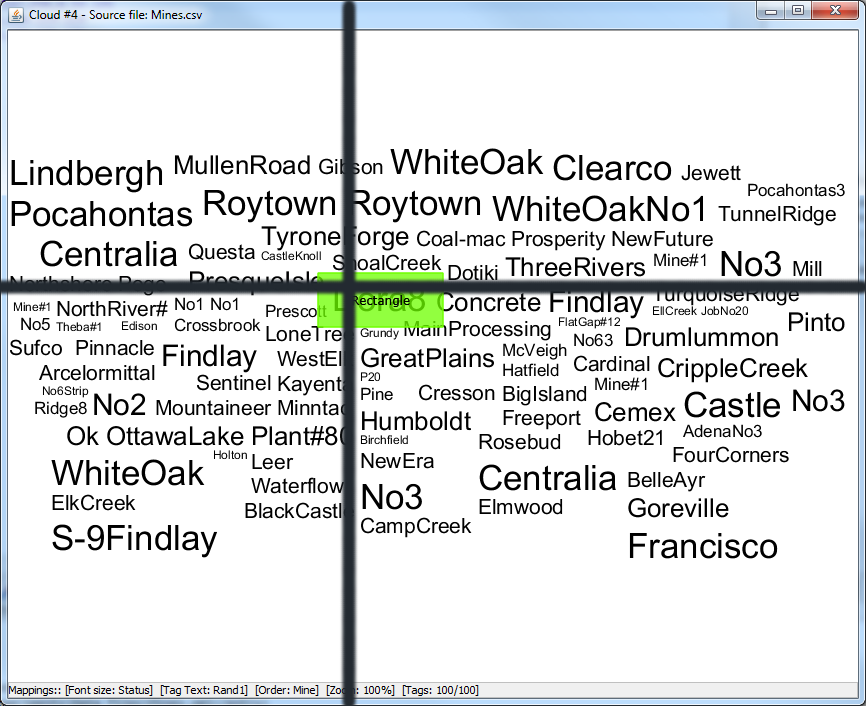
\includegraphics[scale=0.25]{Experiment2/T4/M1Spiral.png}
\end{subfigure}%
\begin{subfigure}{.5\textwidth}
  \centering
  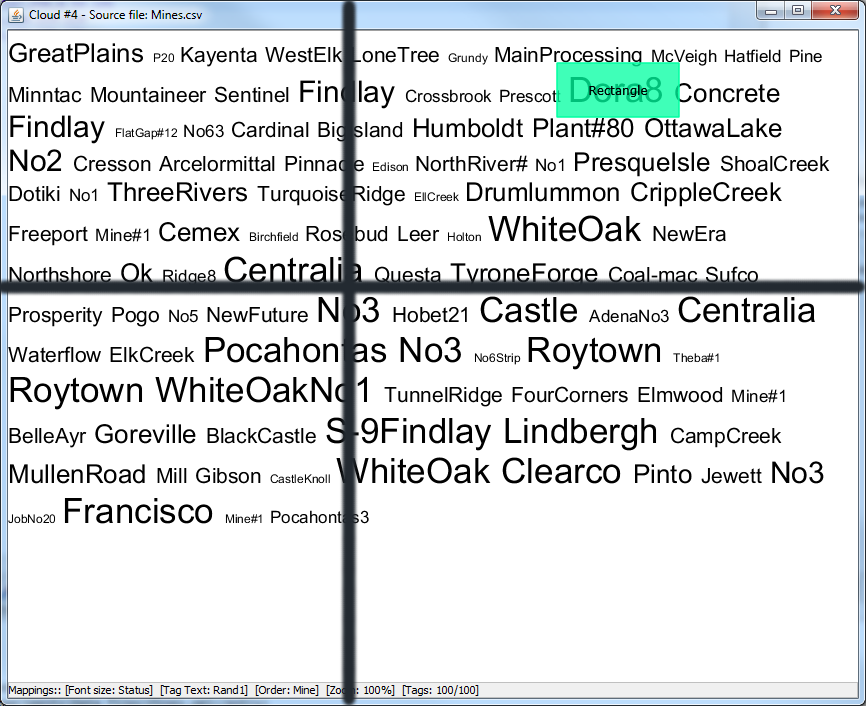
\includegraphics[scale=0.25]{Experiment2/T4/M1Typewriter.png}
\end{subfigure}
\caption{\textit{Experiment two: single font size mapping}}
\end{figure}



\begin{figure}[!htb]
\centering
\begin{subfigure}{.5\textwidth}
  \centering
  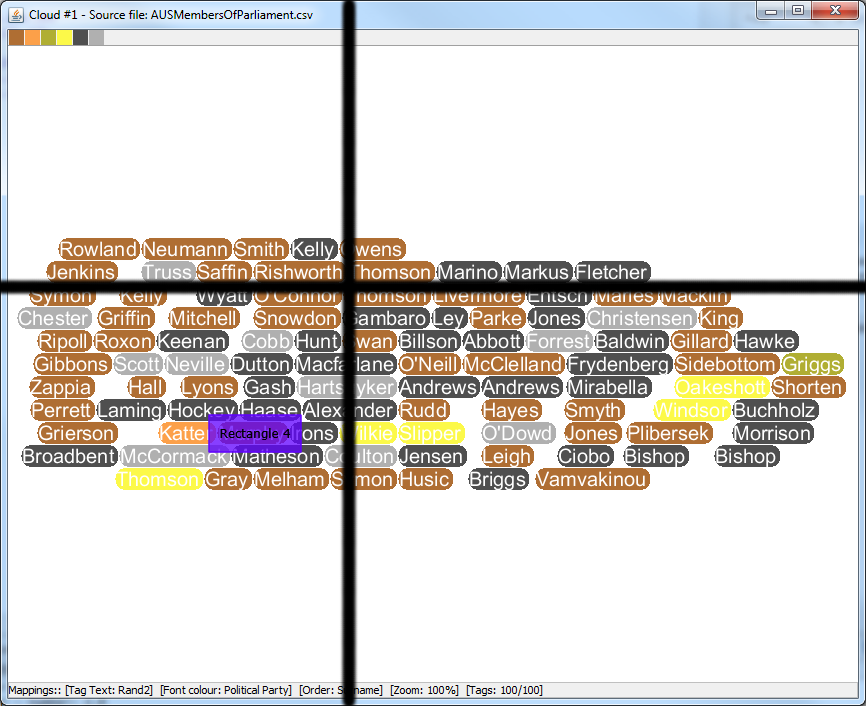
\includegraphics[scale=0.25]{Experiment2/T1/M2Spiral.png}
\end{subfigure}%
\begin{subfigure}{.5\textwidth}
  \centering
 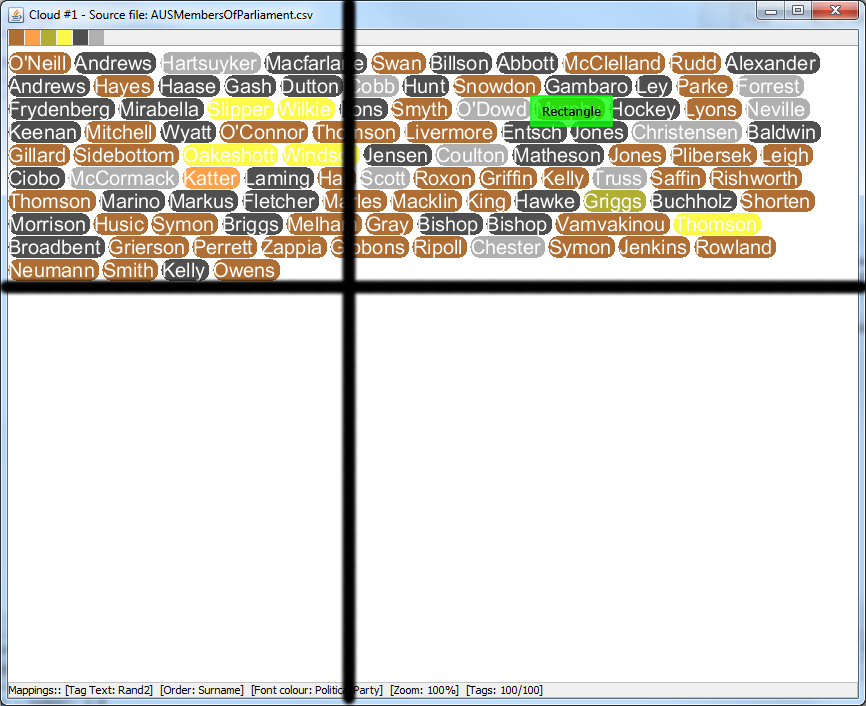
\includegraphics[scale=0.25]{Experiment2/T1/M2Typewriter.png}
\end{subfigure}
\begin{subfigure}{.5\textwidth}
  \centering
  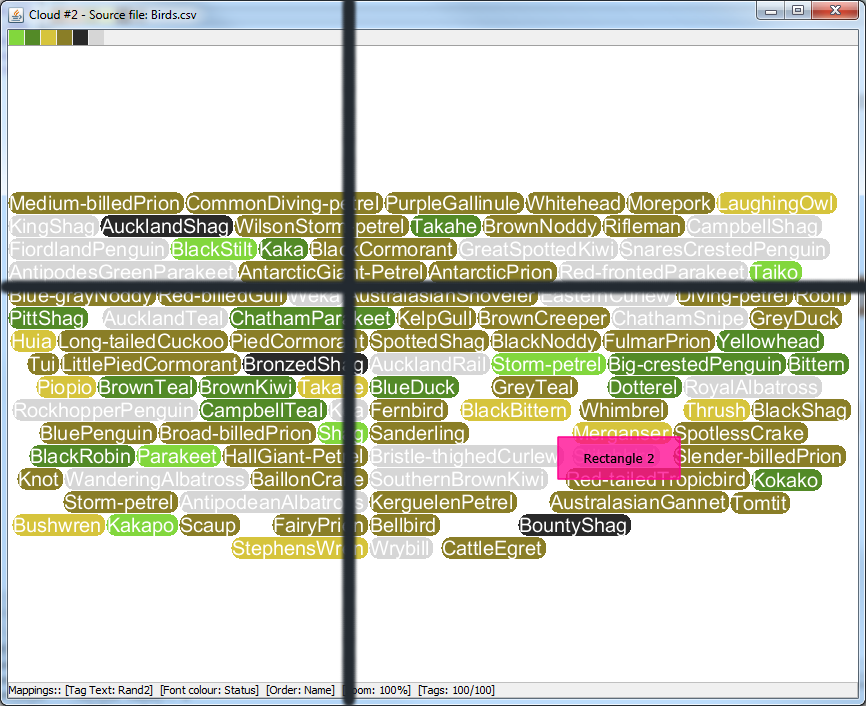
\includegraphics[scale=0.25]{Experiment2/T2/M2Spiral.png}
\end{subfigure}%
\begin{subfigure}{.5\textwidth}
  \centering
 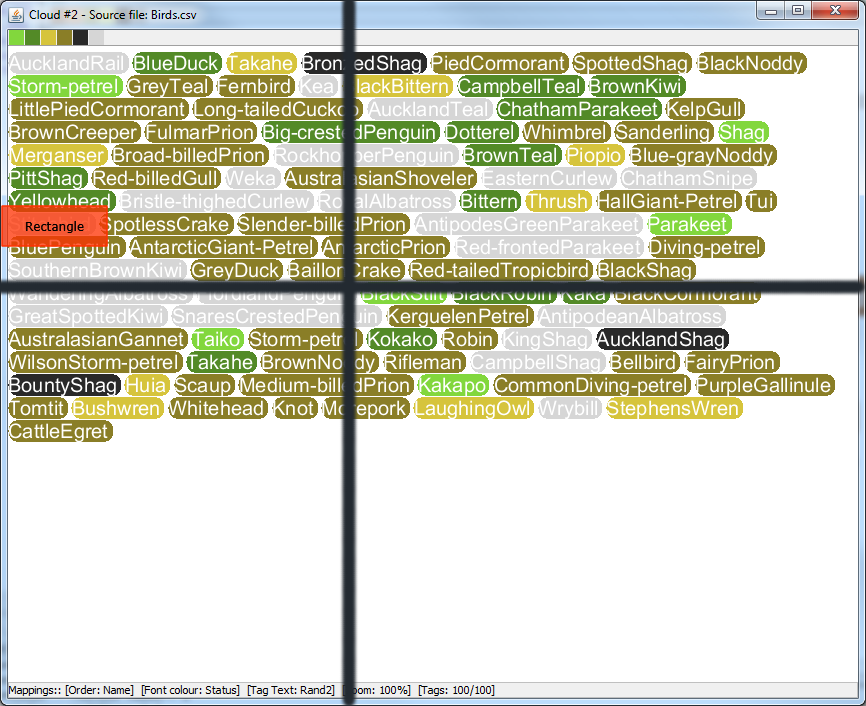
\includegraphics[scale=0.25]{Experiment2/T2/M2Typewriter.png}
\end{subfigure}
\begin{subfigure}{.5\textwidth}
  \centering
  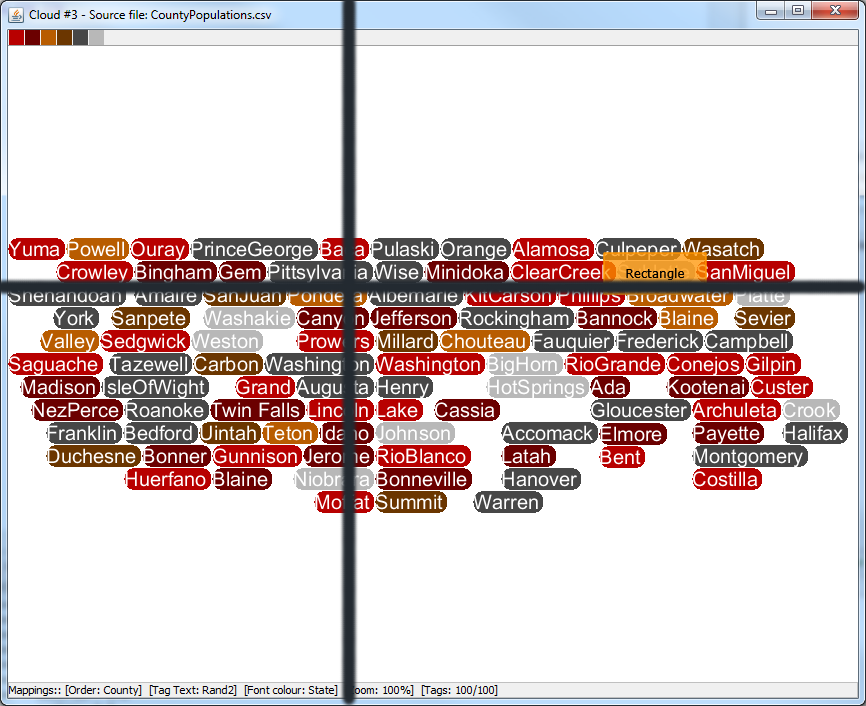
\includegraphics[scale=0.25]{Experiment2/T3/M2Spiral.png}
\end{subfigure}%
\begin{subfigure}{.5\textwidth}
  \centering
 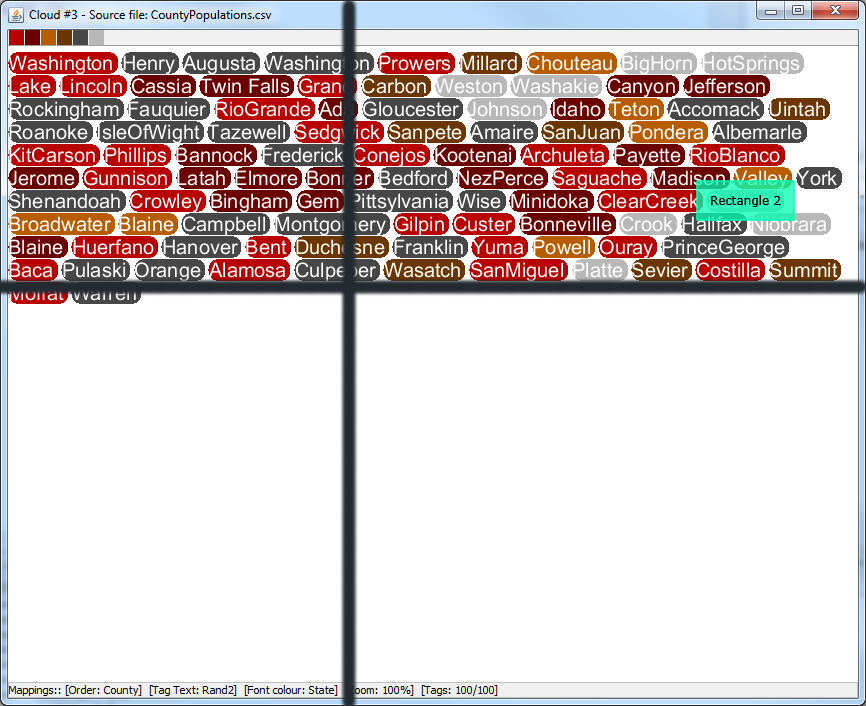
\includegraphics[scale=0.25]{Experiment2/T3/M2Typewriter.png}
\end{subfigure}
\begin{subfigure}{.5\textwidth}
  \centering
  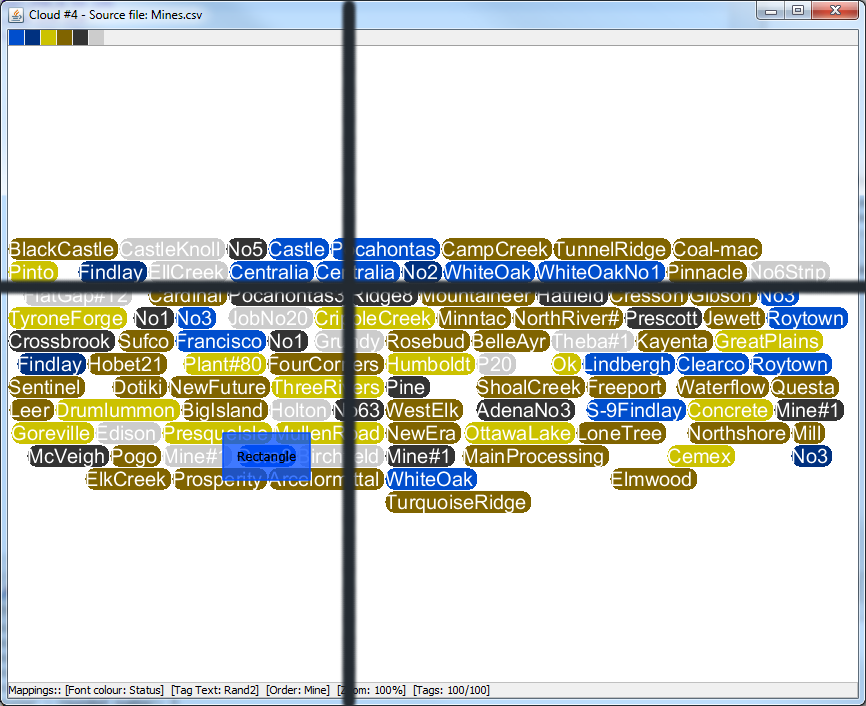
\includegraphics[scale=0.25]{Experiment2/T4/M2Spiral.png}
\end{subfigure}%
\begin{subfigure}{.5\textwidth}
  \centering
 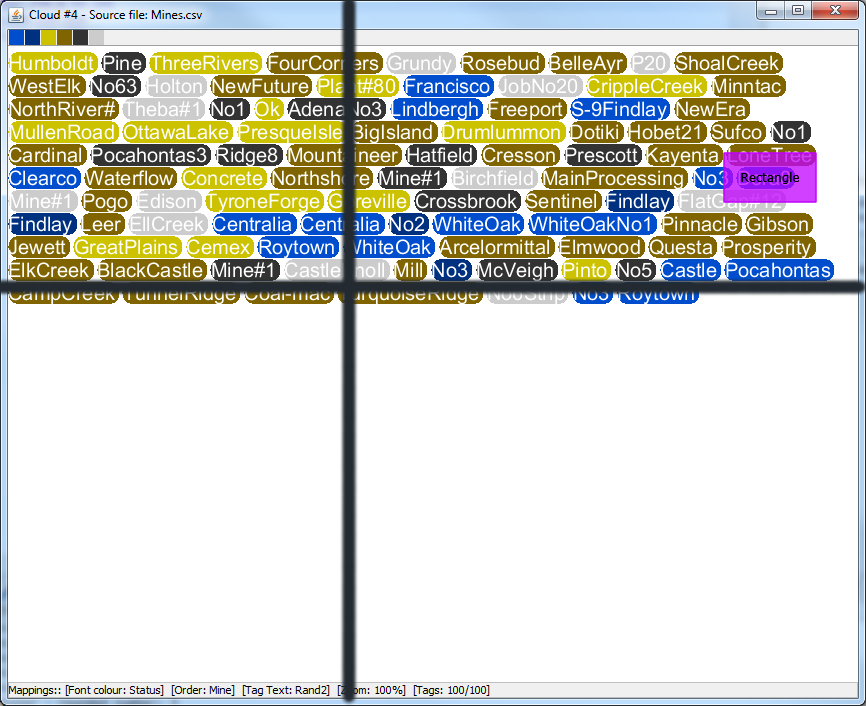
\includegraphics[scale=0.25]{Experiment2/T4/M2Typewriter.png}
\end{subfigure}
\caption{\textit{Experiment two: single colour mapping}}
\end{figure}

\begin{figure}[!htb]
\centering
\begin{subfigure}{.5\textwidth}
  \centering
  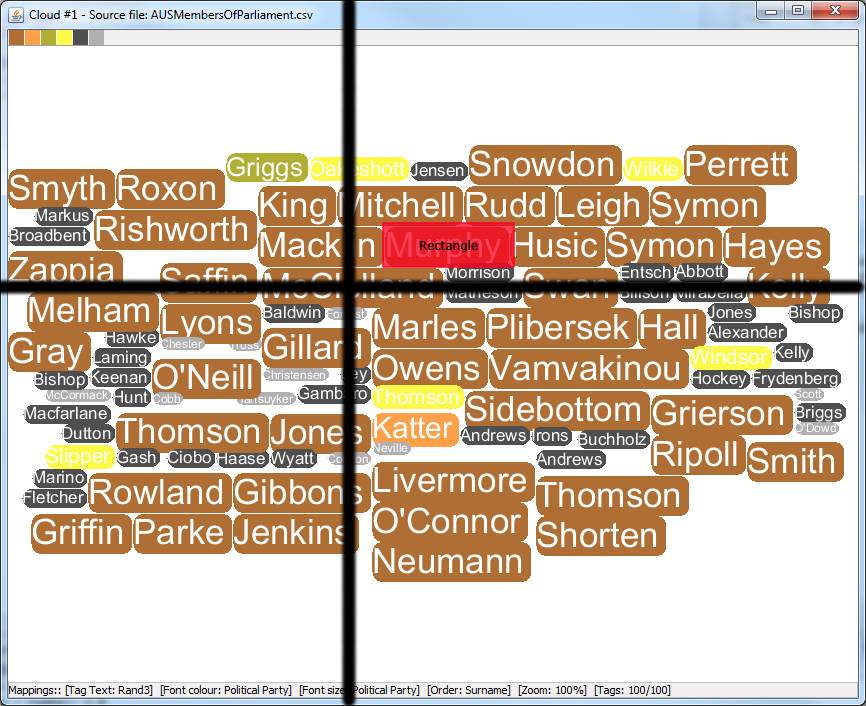
\includegraphics[scale=0.25]{Experiment2/T1/M3Spiral.png}
\end{subfigure}%
\begin{subfigure}{.5\textwidth}
  \centering
 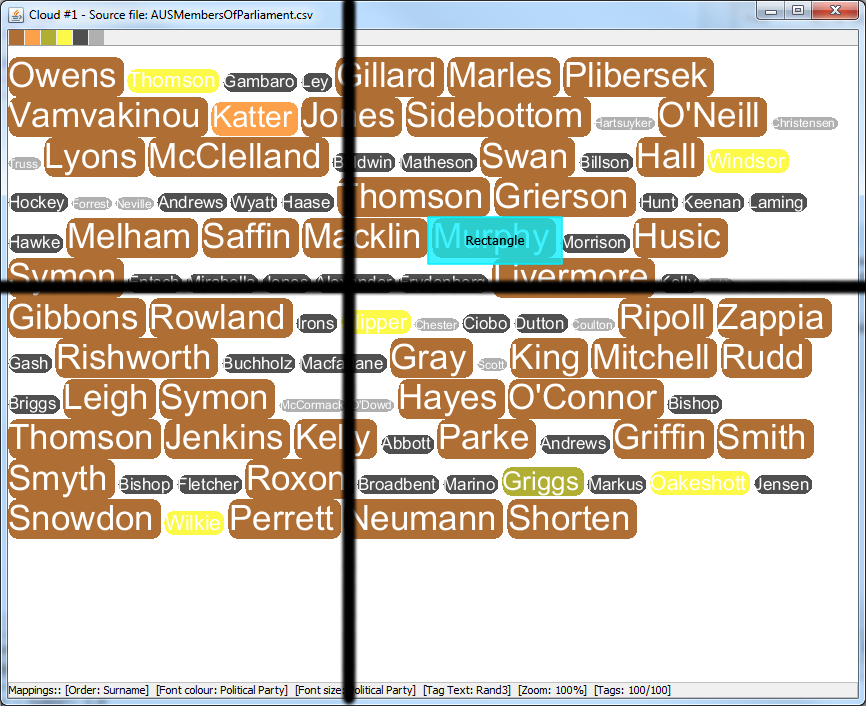
\includegraphics[scale=0.25]{Experiment2/T1/M3Typewriter.png}
\end{subfigure}
\begin{subfigure}{.5\textwidth}
  \centering
  \includegraphics[scale=0.25]{Experiment2/T2/M3Spiral.png}
\end{subfigure}%
\begin{subfigure}{.5\textwidth}
  \centering
 \includegraphics[scale=0.25]{Experiment2/T2/M3Typewriter.png}
\end{subfigure}
\begin{subfigure}{.5\textwidth}
  \centering
  \includegraphics[scale=0.25]{Experiment2/T3/M3Spiral.png}
\end{subfigure}%
\begin{subfigure}{.5\textwidth}
  \centering
 \includegraphics[scale=0.25]{Experiment2/T3/M3Typewriter.png}
\end{subfigure}
\begin{subfigure}{.5\textwidth}
  \centering
  \includegraphics[scale=0.25]{Experiment2/T4/M3Spiral.png}
\end{subfigure}%
\begin{subfigure}{.5\textwidth}
  \centering
 \includegraphics[scale=0.25]{Experiment2/T4/M3Typewriter.png}
\end{subfigure}
\caption{\textit{Experiment two: dual font size and colour mapping}}
\end{figure}




% ------------------------------------------------------------------------

%%% Local Variables: 
%%% mode: latex
%%% TeX-master: "../thesis"
%%% End: 
